%% =========================================================================
%%  AUTOVERSE 3D -- VTU Project Report
%%  Visvesvaraya Technological University, Belagavi
%%  Department of Computer Science & Engineering
%%  Government Engineering College, Hassan - 573201
%%
%%  Compile with:   pdflatex AutoVerse_3D_Project_Report.tex   (run 3 times)
%%  or:             latexmk -pdf AutoVerse_3D_Project_Report.tex
%% =========================================================================
\documentclass[12pt,a4paper]{report}

\usepackage[a4paper,top=24mm,bottom=24mm,left=24mm,right=20mm,includehead,includefoot,headheight=18pt,headsep=12pt,footskip=14pt]{geometry}
\usepackage[T1]{fontenc}
\usepackage[utf8]{inputenc}
\usepackage{mathptmx}
\usepackage[scaled=.90]{helvet}
\usepackage{courier}
\usepackage{graphicx}
\usepackage{xcolor}
\usepackage{amsmath,amssymb}
\usepackage{listings}
\usepackage{tabularx}
\usepackage{array}
\usepackage{fancyhdr}
\usepackage{eso-pic}
\usepackage{titlesec}
\usepackage{titletoc}
\usepackage{enumitem}
\usepackage[labelfont=bf]{caption}
\usepackage{adjustbox}
\usepackage{setspace}
\usepackage{url}
\urlstyle{same}
\DeclareUrlCommand\code{\urlstyle{tt}}
\usepackage{tikz}
\usetikzlibrary{calc,positioning,shapes.geometric,arrows.meta,fit,backgrounds}

\setstretch{1.12}
\setlist{itemsep=2pt,topsep=4pt,parsep=0pt}
\setlength{\parindent}{0pt}
\setlength{\parskip}{6pt}
\emergencystretch=2em

% ----------------------------------------------------------------- colors
\definecolor{vtumaroon}{RGB}{128,0,0}
\definecolor{vtublue}{RGB}{20,60,140}
\definecolor{darkslate}{RGB}{30,41,59}
\definecolor{codegray}{RGB}{245,247,250}

% ----------------------------------------------------- image with fallback
\newcommand{\safeimg}[2]{%
  \IfFileExists{#1}{\includegraphics[#2]{#1}}{%
    \fbox{\parbox[c][4cm][c]{0.6\linewidth}{\centering\scriptsize\ttfamily Missing image:\\\detokenize{#1}}}}}

% ------------------------------------------------------------ code listings
\lstset{
  backgroundcolor=\color{codegray},
  basicstyle=\ttfamily\footnotesize,
  breaklines=true,
  frame=single,
  rulecolor=\color{black!30},
  numbers=left,
  numberstyle=\tiny\color{gray},
  captionpos=b,
  keywordstyle=\bfseries\color{vtublue},
  commentstyle=\itshape\color{green!50!black},
  stringstyle=\color{vtumaroon},
  xleftmargin=1.6em,
  aboveskip=8pt,
  belowskip=4pt
}
\AtBeginDocument{\numberwithin{lstlisting}{chapter}}
\renewcommand{\lstlistingname}{Listing}

% --------------------------------------------------- page border on all pages
\AddToShipoutPictureBG{%
  \begin{tikzpicture}[remember picture, overlay]
    \draw[line width=1.5pt, color=black] ($(current page.north west)+(14mm,-14mm)$) rectangle ($(current page.south east)+(-14mm,14mm)$);
  \end{tikzpicture}%
}

% ------------------------------------------------------------ header/footer
\pagestyle{fancy}
\fancyhf{}
\fancyhead[L]{\small\textbf{\color{darkslate}AUTOVERSE 3D: AUTOMOTIVE DESIGN \& SIMULATION}}
\fancyhead[R]{\small\textbf{\color{darkslate}2025-26}}
\fancyfoot[L]{\small\color{darkslate}Dept. of CSE, GEC, Hassan}
\fancyfoot[R]{\small\textbf{\color{darkslate}Page \thepage}}
\renewcommand{\headrule}{\color{vtumaroon}\hrule width\headwidth height 1.2pt \vskip 1pt \hrule width\headwidth height 0.4pt}
\renewcommand{\footrule}{\color{vtumaroon}\hrule width\headwidth height 0.4pt \vskip 1pt \hrule width\headwidth height 1.2pt}
\fancypagestyle{plain}{%
  \fancyhf{}
  \fancyhead[L]{\small\textbf{\color{darkslate}AUTOVERSE 3D: AUTOMOTIVE DESIGN \& SIMULATION}}
  \fancyhead[R]{\small\textbf{\color{darkslate}2025-26}}
  \fancyfoot[L]{\small\color{darkslate}Dept. of CSE, GEC, Hassan}
  \fancyfoot[R]{\small\textbf{\color{darkslate}Page \thepage}}
  \renewcommand{\headrule}{\color{vtumaroon}\hrule width\headwidth height 1.2pt \vskip 1pt \hrule width\headwidth height 0.4pt}
  \renewcommand{\footrule}{\color{vtumaroon}\hrule width\headwidth height 0.4pt \vskip 1pt \hrule width\headwidth height 1.2pt}
}

% ----------------------------------------------------------------- headings
\titleformat{\chapter}[display]
  {\bfseries}
  {\Large Chapter \thechapter}
  {8pt}
  {\centering\LARGE}
\titlespacing*{\chapter}{0pt}{0pt}{18pt}
\titleformat{\section}{\bfseries\large}{\thesection}{0.8em}{\MakeUppercase}
\titlespacing*{\section}{0pt}{14pt}{6pt}
\titleformat{\subsection}{\bfseries\normalsize}{\thesubsection}{0.8em}{}
\titlespacing*{\subsection}{0pt}{10pt}{4pt}

% -------------------------------------------------------- contents formatting
\renewcommand{\contentsname}{TABLE OF CONTENTS}
\renewcommand{\listfigurename}{LIST OF FIGURES}
\renewcommand{\listtablename}{LIST OF TABLES}
\titlecontents{chapter}[0em]{\addvspace{6pt}\bfseries}{\contentslabel[\thecontentslabel.]{1.8em}}{}{\titlerule*[0.7pc]{.}\contentspage}
\titlecontents{section}[1.8em]{}{\contentslabel{2.4em}}{}{\titlerule*[0.7pc]{.}\contentspage}
\titlecontents{subsection}[4.2em]{}{\contentslabel{3.2em}}{}{\titlerule*[0.7pc]{.}\contentspage}
\titlecontents{figure}[0em]{}{Figure~\thecontentslabel:\quad}{}{\titlerule*[0.7pc]{.}\contentspage}
\titlecontents{table}[0em]{}{Table~\thecontentslabel:\quad}{}{\titlerule*[0.7pc]{.}\contentspage}

% ----------------------------------------------------------- reference items
\newcommand{\refitem}[2]{\par\noindent\hangindent=2.6em\hangafter=1 [#1]\hspace{0.9em}#2\par\vspace{2pt}}

% ------------------------------------------------------------ TikZ helpers
\tikzset{
  arrow/.style={-{Latex[length=2.2mm]}, thick},
  box/.style={rectangle, draw=black, fill=blue!5, thick, align=center, rounded corners, minimum height=1.0cm, font=\small},
  secbox/.style={rectangle, draw=vtumaroon, fill=red!5, thick, align=center, rounded corners, minimum height=1.0cm, font=\small}
}
\newcommand{\actor}[3]{%
  \begin{scope}[shift={(#1,#2)}]
    \draw[thick] (0,0.55) circle (0.2);
    \draw[thick] (0,0.35)--(0,-0.15) (-0.3,0.2)--(0.3,0.2) (0,-0.15)--(-0.25,-0.6) (0,-0.15)--(0.25,-0.6);
    \node[font=\small\bfseries,below] at (0,-0.6) {#3};
  \end{scope}}

\begin{document}

% =========================================================================
% TITLE PAGE
% =========================================================================
\thispagestyle{empty}
\begin{center}
  {\bfseries\large VISVESVARAYA TECHNOLOGICAL UNIVERSITY}\\[0.15cm]
  {\bfseries\normalsize ``JNANA SANGAMA'', BELAGAVI -- 590 018}\\[0.5cm]
  \safeimg{figures/vtu_logo.png}{width=2.4cm}\\[0.5cm]
  {\normalsize PROJECT REPORT ON}\\[0.3cm]
  {\bfseries\Large\color{vtublue} ``AUTOVERSE 3D: HIGH-FIDELITY WEB-BASED 3D AUTOMOTIVE DESIGN, PARAMETRIC B-REP COACHWORK GENERATION, AND REAL-TIME AERODYNAMIC SIMULATION PLATFORM''}\\[0.5cm]
  {\normalsize Submitted in partial fulfilment of the requirement\\for the award of the degree of}\\[0.3cm]
  {\bfseries\normalsize BACHELOR OF ENGINEERING}\\[0.1cm]
  {\bfseries\normalsize IN}\\[0.1cm]
  {\bfseries\normalsize COMPUTER SCIENCE AND ENGINEERING}\\[0.5cm]

  \textbf{\underline{Submitted By}}\\[0.25cm]
  {\color{vtublue}
  \renewcommand{\arraystretch}{1.25}
  \begin{tabular}{lcl}
    Bhanupriya N R    & : & 4GH24CS019 \\
    Chaithanya B N    & : & 4GH24CS026 \\
    Charan Gowda H D  & : & 4GH24CS034 \\
    Deekshith G       & : & 4GH24CS040 \\
  \end{tabular}}\\[0.5cm]

  \textbf{\underline{Under the Guidance of}}\\[0.2cm]
  \textbf{Dr. Mahendra G}\\
  Guide\\[0.5cm]

  \textbf{DEPARTMENT OF COMPUTER SCIENCE \& ENGINEERING}\\
  \textbf{GOVERNMENT ENGINEERING COLLEGE, HASSAN -- 573201}\\
  \textbf{2025-26}
\end{center}
\newpage

% =========================================================================
% CERTIFICATE (NO Project Co-Ordinator, per explicit instructions)
% =========================================================================
\thispagestyle{empty}
\begin{center}
  \textbf{\large GOVERNMENT ENGINEERING COLLEGE HASSAN -- 573 201}\\
  \small Affiliated to VTU, Belagavi \& Approved by AICTE, New Delhi\\[0.05cm]
  \textbf{\normalsize DEPARTMENT OF COMPUTER SCIENCE \& ENGINEERING}\\[0.3cm]
  \safeimg{figures/karnataka_emblem.png}{width=2.5cm}\\[0.4cm]
  \textbf{\Large CERTIFICATE}\\[0.2cm]
\end{center}

{\sloppy\setlength{\parindent}{1.5em}
Certified that the Project work entitled \textbf{``AUTOVERSE 3D: HIGH-FIDELITY WEB-BASED 3D AUTOMOTIVE DESIGN, PARAMETRIC B-REP COACHWORK GENERATION, AND REAL-TIME AERODYNAMIC SIMULATION PLATFORM''} carried out by \textbf{Bhanupriya N R (4GH24CS019), Chaithanya B N (4GH24CS026), Charan Gowda H D (4GH24CS034) and Deekshith G (4GH24CS040)}, bonafide students of \textbf{Government Engineering College Hassan}, in partial fulfilment for the award of \textbf{Bachelor of Engineering in Computer Science and Engineering} of the \textbf{Visvesvaraya Technological University, Belagavi} during the academic year 2025-2026. It is certified that all corrections and suggestions indicated during internal evaluation have been incorporated in the report. The Project report has been approved as it satisfies the academic requirements in respect of Project work prescribed for the said Degree.\par}
\vspace{1.0cm}

\noindent
\begin{tabular}{p{7.5cm}p{7.5cm}}
\textbf{Dr. Mahendra G} & \textbf{Dr. Vani V G}\\
Guide & HoD, Dept. of CSE\\[1.5cm]
\multicolumn{2}{c}{\textbf{Dr. Girish D P}}\\
\multicolumn{2}{c}{Principal}
\end{tabular}\\[1.0cm]

\noindent
\textbf{Name of the Examiners} \hfill \textbf{Signature with Date}\\[0.4cm]
1. ..................................................... \hfill .....................................................\\[0.4cm]
2. ..................................................... \hfill .....................................................
\newpage
\ClearShipoutPictureBG

% =========================================================================
% DECLARATION
% =========================================================================
\thispagestyle{empty}
\begin{center}
  \textbf{\Large DECLARATION}\\[1.0cm]
\end{center}

{\sloppy\setlength{\parindent}{1.5em}
We, \textbf{BHANUPRIYA N R, CHAITHANYA B N, CHARAN GOWDA H D and DEEKSHITH G}, students of B.E., \textbf{GOVERNMENT ENGINEERING COLLEGE, HASSAN} bearing USNs \textbf{4GH24CS019, 4GH24CS026, 4GH24CS034 and 4GH24CS040} respectively, hereby declare that the Project entitled \textbf{``AUTOVERSE 3D: HIGH-FIDELITY WEB-BASED 3D AUTOMOTIVE DESIGN, PARAMETRIC B-REP COACHWORK GENERATION, AND REAL-TIME AERODYNAMIC SIMULATION PLATFORM''} has been carried out by us under the supervision of our Guide, \textbf{DR. MAHENDRA G}, Department of Computer Science \& Engineering, Government Engineering College, Hassan.\par}

\vspace{0.4cm}
{\setlength{\parindent}{1.5em}
We have submitted this report in partial fulfilment of the requirements for the award of the Degree of Bachelor of Engineering in Computer Science \& Engineering by the Visvesvaraya Technological University, Belagavi during the academic year 2025-2026. This report has not been submitted to any other Organization or University for the award of any degree or certificate.\par}

\vspace{1.2cm}
\noindent
\textbf{Date:} November 24, 2026 \hfill \textbf{Project Associates:}\\[0.2cm]
\textbf{Place:} Hassan \hfill BHANUPRIYA N R\\
\null \hfill CHAITHANYA B N\\
\null \hfill CHARAN GOWDA H D\\
\null \hfill DEEKSHITH G
\newpage

% =========================================================================
% ACKNOWLEDGEMENT
% =========================================================================
\pagenumbering{roman}
\setcounter{page}{1}

\begin{center}
  \textbf{\Large ACKNOWLEDGEMENT}\\[0.6cm]
\end{center}

We consider it a privilege to whole-heartedly express our gratitude and respect to each and every one who guided and helped us in the successful completion of this Project Report.

We are very thankful to the Principal, \textbf{Dr. Girish D P}, for being kind enough to provide us an opportunity to work on a project of this technical depth and engineering scope in this institution.

We also express our sincere gratitude to \textbf{Dr. Vani V G}, Head of the Department of Computer Science and Engineering, for her co-operation, academic leadership and continuous encouragement throughout the duration of our project work.

We would like to specially mention the profound influence and constructive guidance provided by \textbf{Dr. Mahendra G}, Project Guide, for his invaluable technical insights, critical feedback and steadfast co-operation during our venture, making this project an inspiring and rigorous learning experience.

We would also like to thank our parents and family members for their enduring moral support and blessings, as well as our dear classmates and friends for their camaraderie and assistance.

Finally, it is our pleasure to extend our appreciation to all the teaching, technical and laboratory staff members of the Department of Computer Science and Engineering, Government Engineering College, Hassan.

\vspace{0.8cm}
\hfill \textbf{Project Associates:}\\[0.2cm]
\null \hfill Bhanupriya N R (4GH24CS019)\\
\null \hfill Chaithanya B N (4GH24CS026)\\
\null \hfill Charan Gowda H D (4GH24CS034)\\
\null \hfill Deekshith G (4GH24CS040)
\newpage

% =========================================================================
% ABSTRACT
% =========================================================================
\begin{center}
  \textbf{\Large ABSTRACT}\\[0.6cm]
\end{center}

\begin{spacing}{1.0}
Traditional automotive computer-aided design (CAD) suites and computational fluid dynamics (CFD) pipelines are computationally massive, reliant on local workstation installations, and fundamentally decoupled from real-time interactive design environments. Automotive styling studios and engineering teams face substantial latency between conceptual styling, 3D parameter modification, and aerodynamic validation, while web-based vehicle configurators routinely offer only pre-rendered static assets or fragile, unclosed polygonal meshes prone to visual tearing and non-manifold boundary errors.

This project presents \textbf{AutoVerse 3D}, an integrated, high-fidelity, web-based 3D automotive design, parametric coachwork synthesis, and real-time aerodynamic simulation platform. The platform operates on a dual-tier architecture:

\textbf{Tier 1 -- WebGL Parametric Geometry and Visual Engine:} Built upon Three.js and React Three Fiber, the client introduces a Phase-C V2 Coachwork Generator that synthesizes watertight, manifold 3D body shells via parametric closed cross-section lofting. The geometry engine supports 24 typed Brand Design Languages (including Porsche, Lamborghini, Ferrari, McLaren, BMW, and Nissan), enforcing distinct styling proportions, front splitter and rear diffuser attachments, and contact-verified wheel assemblies (rim diameter, track offset, and camber controls) that sit precisely on the road surface with zero ground penetration ($y \ge 0$). High-fidelity physically based rendering (PBR) shaders simulate multi-coat metallic clearcoat paint, anisotropic carbon fiber weaves, and optical glass refractions. A responsive phone landscape workstation interface ensures seamless touch and desktop usability across extreme viewport aspect ratios.

\textbf{Tier 2 -- Real-Time Aerodynamic Simulation and Cloud Persistence:} The simulation kernel computes aerodynamic coefficients ($C_d$, $C_l$) and vehicle downforce via an empirical component-buildup formulation anchored to standardized aerodynamic literature, including the Ahmed $25^\circ$ reference body and the DrivAer realistic automotive benchmark. A FastAPI/PostgreSQL cloud backend provides versioned project persistence, multi-tenant workspace management, and asset validation gates. A strict \textit{Zero-Fabrication Charter} and automated provenance audit gate prohibit misleading claims of physical validation, labeling procedural geometries and analytic estimates with honest, transparent classifications.

Comprehensive automated verification across all tiers---56 frontend Vitest suites comprising 386 unit/integration tests and 3 backend Pytest suites comprising 16 API/database tests (402 total tests)---passed with a 100\% green continuous integration (CI) run on GitHub Actions, proving the architectural stability, geometric manifoldness, and mathematical integrity of the system.
\end{spacing}

\vspace{0.4cm}
\noindent\textbf{Keywords:} WebGL 3D CAD, Parametric Coachwork Engine, Computational Fluid Dynamics (CFD), Three.js, React Three Fiber, Brand Design Language, Aerodynamic Drag Estimation, Ahmed Reference Body, Zero Geometry Fabrication, FastAPI.
\newpage

% =========================================================================
% TABLE OF CONTENTS, LIST OF FIGURES, LIST OF TABLES
% =========================================================================
\tableofcontents
\newpage
\listoffigures
\vspace{0.8cm}
\begingroup
\let\clearpage\relax
\let\cleardoublepage\relax
\listoftables
\endgroup
\newpage

% =========================================================================
% CHAPTER 1
% =========================================================================
\pagenumbering{arabic}
\setcounter{page}{1}

\chapter{INTRODUCTION}

\section{Project Overview}
The automotive design and manufacturing industry has historically operated with heavy, siloed computer-aided design (CAD) software packages and separate, computationally expensive computational fluid dynamics (CFD) simulation environments. Transitioning an automobile concept from a designer's initial artistic vision to a structurally sound, aerodynamically evaluated 3D digital twin typically requires days or weeks of manual mesh repair, surface reconstruction, and solver configuration on high-performance compute clusters.

On the consumer and enthusiast front, web-based vehicle configurators provided by automobile manufacturers have remained largely cosmetic, relying on pre-rendered 2D raster image sequences or simplified 3D models with static polygon geometry. These applications lack parametric geometric malleability, real-time physics feedback, and mechanical packaging intelligence. Furthermore, existing procedural geometry algorithms on the web often suffer from degenerate triangles, unclosed profile curves, flipped surface normals, and detached floating meshes.

\textbf{AutoVerse 3D} is an autonomous, web-native 3D automotive engineering and styling studio that bridges parametric CAD modeling, physically based rendering (PBR), and real-time aerodynamic simulation directly within standard web browsers. Operating without external CAD plugins or proprietary runtime dependencies, AutoVerse 3D provides a componentized 3D geometry engine capable of synthesizing watertight vehicle coachwork based on distinct brand design languages, coupled with an analytic aerodynamic solver that provides immediate drag, downforce, and airflow telemetry during interactive modifications.

\section{Problem Statement}
Contemporary automotive styling and web-based 3D design platforms suffer from several fundamental engineering deficiencies:
\begin{enumerate}
    \item \textbf{High Entry Barrier and Software Weight:} Traditional automotive CAD/CAM tools (e.g., Siemens NX, CATIA) are desktop-bound, licensing-heavy, and require substantial computing hardware, preventing cross-device collaboration, web accessibility, and lightweight rapid prototyping.
    \item \textbf{Geometric Defects in Procedural Web Models:} Existing web-based procedural geometry generators frequently produce non-manifold boundaries, self-intersecting hulls, jagged polygon spikes, and detached aerodynamic components (such as floating rear wings and misaligned wheel hubs).
    \item \textbf{Decoupled Aerodynamic Feedback:} Designers adjust vehicle ride height, camber, splitters, and spoilers without real-time insight into the aerodynamic trade-offs ($C_d$, downforce, and induced drag), relying instead on delayed batch CFD runs.
    \item \textbf{Deceptive Provenance and Data Fabrication:} Many computational tools label simplified numerical approximations as ``physically validated'' or fabricate realistic-looking aerodynamic data without disclosing true mathematical origins or adhering to standard literature benchmarks.
    \item \textbf{Mobile and Cross-Platform Fragility:} Complex 3D viewports and CAD control panels collapse or display fatal WebGL context crashes (black screens) when accessed on mobile touchscreens or non-standard aspect ratios.
\end{enumerate}

\section{Scope of the Project}
The scope of AutoVerse 3D encompasses a full-stack, browser-based automotive engineering ecosystem compliant with VTU Bachelor of Engineering project standards [1]:
\begin{itemize}
    \item \textbf{Parametric B-Rep Coachwork Engine:} An authentic 3D geometry generation pipeline implementing closed cross-section lofting, wheel-arch boolean cutouts, and separable component hierarchies across 24 distinct automotive brands.
    \item \textbf{Real-Time Aerodynamic Solver:} A component-buildup analytical aerodynamic engine that estimates vehicle drag ($C_d$), lift ($C_l$), and aerodynamic balance, benchmarked against the Ahmed reference body and DrivAer literature.
    \item \textbf{High-Fidelity Studio Rendering:} A Three.js/WebGL presentation subsystem featuring physically based clearcoat car paint, metallic flakes, anisotropic carbon fiber composites, and dynamic studio HDRI lighting.
    \item \textbf{Responsive Phone Landscape Workstation:} A mobile-responsive user interface optimized for landscape smartphone viewports ($800\times360$ to $896\times414$) as well as desktop ultrawide monitors.
    \item \textbf{Cloud Persistence and Engineering Export:} A Python FastAPI service with SQLite/PostgreSQL persistence, offering vehicle CRUD operations, revision history, and standard multi-format exports (GLTF, Wavefront OBJ, DXF 2D profiles, and CSV telemetry).
    \item \textbf{Honest Provenance and Quality Gates:} Automated testing suites that enforce watertightness, non-zero component contact, and strict labeling of procedural outputs under an explicit Zero-Fabrication Charter.
\end{itemize}

\section{Challenges in 3D Automobile Design and Simulation}
\begin{enumerate}
    \item \textbf{Watertight Lofting under Dynamic Curvature:} Lofting complex automotive body profiles requires continuous mathematical smoothness ($G^1/G^2$ continuity) and closed cross-sections to eliminate vertex spikes and degenerate triangles.
    \item \textbf{Browser Memory Management:} Sequentially switching across a 50-vehicle catalog in WebGL can rapidly cause GPU texture and geometry buffer leaks, requiring rigorous disposal of Three.js geometries, materials, and canvas contexts.
    \item \textbf{Analytic vs. Full-Navier-Stokes Accuracy:} Balancing real-time sub-second response times with physically meaningful drag estimation requires robust semi-empirical formulations that reflect real aerodynamic trends without hallucinating CFD convergence.
    \item \textbf{Mobile Touch Ergonomics:} Managing complex multi-axis 3D orbit controls alongside dense engineering parameters (camber, rim diameter, ride height, wing angle) within constrained mobile screen real estate.
\end{enumerate}

\section{Objectives of the Project}
\begin{itemize}
    \item To design and implement a web-native parametric geometry engine that generates manifold, watertight 3D automotive coachwork without polygon spikes or floating components.
    \item To develop a typed \textbf{Brand Design Language (BDL)} framework covering 24 distinct manufacturers to ensure brand-faithful vehicle silhouettes and proportion rules.
    \item To incorporate real-time kinematic wheel assembly controls (camber angle, rim diameter, offset track spacer) that maintain exact road-contact invariants ($y \ge 0$).
    \item To formulate a real-time aerodynamic simulation kernel based on the component-buildup method, calibrated against standard Ahmed body and DrivAer experimental benchmarks.
    \item To build a responsive, production-level studio workstation supporting desktop ultrawide and mobile phone landscape orientations with graceful WebGL error recovery.
    \item To establish a cloud persistence backend using FastAPI with database migrations, multi-tenant isolation, and multi-format engineering exports.
    \item To implement a strict \textbf{Honest Provenance Charter} and verify the entire system empirically through comprehensive automated CI test suites.
\end{itemize}

% =========================================================================
% CHAPTER 2
% =========================================================================
\chapter{LITERATURE SURVEY}

\section{Related Works}
Automotive styling, 3D surface modeling, and aerodynamic evaluation have evolved across several key software and computational domains.

\subsection{Commercial Automotive CAD/CAM Suites}
High-end engineering environments such as Siemens NX, Dassault Systèmes CATIA, and Autodesk Alias represent the industrial standard for Class-A surface modeling and mechanical packaging [2]. While these tools provide micro-millimeter precision and non-uniform rational B-spline (NURBS) mathematics, they are closed-source, desktop-bound, computationally intensive, and prohibitively expensive for lightweight design reviews, rapid concept exploration, and web deployment.

\subsection{WebGL Vehicle Configurators and Visualizers}
Consumer-facing vehicle configurators built on WebGL or streaming engines (e.g., Unreal Engine Pixel Streaming) emphasize photorealistic rendering for commercial sales [4]. However, these applications rely on static pre-authored polygonal assets (GLTF or FBX). They do not generate geometry dynamically, lack parametric coachwork deformation, and provide zero engineering or aerodynamic computation.

\subsection{Aerodynamic Simulation and Drag Estimation Methods}
Full 3D computational fluid dynamics typically employs Reynolds-Averaged Navier-Stokes (RANS) or Large Eddy Simulation (LES) formulations using solvers such as OpenFOAM [7]. While RANS provides detailed boundary-layer resolution, simulating a single automotive geometry requires hours of cluster computation and millions of grid cells, making it unviable for interactive design. To overcome this, researchers developed standardized empirical references, notably the Ahmed Reference Body [3] and the DrivAer Model [16], allowing component-buildup aerodynamic models to estimate drag coefficients ($C_d$) analytically in real time based on vehicle frontal area, ground clearance, and rear slant angles [13].

\subsection{Web-Native Parametric Geometry Kernels}
Recent advancements in WebAssembly and TypeScript have brought parametric computational geometry to browsers. Frameworks such as OpenCASCADE.js and Manifold CAD demonstrate the viability of client-side boundary representation (B-Rep). AutoVerse 3D extends these principles to specialized automotive archetypes, utilizing closed cross-sectional lofting and hierarchical scene graphs in Three.js [10].

\section{Comparative Analysis}

\begin{table}[htbp]
\centering
\small
\caption{Comparative Analysis of Automotive 3D Design and Simulation Platforms}
\label{tab:lit_comparison}
\renewcommand{\arraystretch}{1.3}
\begin{tabularx}{\textwidth}{|>{\raggedright\arraybackslash}p{2.6cm}|>{\raggedright\arraybackslash}X|>{\raggedright\arraybackslash}X|>{\raggedright\arraybackslash}X|>{\raggedright\arraybackslash}X|}
\hline
\textbf{Feature} & \textbf{Desktop CAD (CATIA/Alias)} & \textbf{Commercial Web Configurator} & \textbf{OpenFOAM CFD} & \textbf{AutoVerse 3D (Proposed)} \\
\hline
Deployment & Native Desktop & Web Browser & Linux HPC Cluster & Web Browser (Mobile \& Desktop) \\
\hline
Geometry Generation & Manual NURBS curves & Static pre-rendered meshes & Pre-meshed volume grid & Parametric B-Rep coachwork lofting \\
\hline
Simulation Speed & None (requires export) & None & Hours / Days per run & Real-time ($< 50$ ms analytic update) \\
\hline
Brand Design Rules & Manual authoring & Model-specific meshes & N/A & 24 Typed Brand Design Languages \\
\hline
Aerodynamic Coupling & Decoupled & None & Coupled via offline mesh & Real-time component buildup ($C_d, C_l$) \\
\hline
Mobile Landscape UI & None & Limited touch support & CLI / Scripting only & Specialized touch HUD ($800\times360$) \\
\hline
Provenance Charter & Proprietary & Commercial marketing & Academic convergence logs & Transparent analytic / procedural labeling \\
\hline
Multi-Format Export & STEP, IGES & None (Images only) & VTK, OpenFOAM raw & GLTF, Wavefront OBJ, DXF, CSV \\
\hline
\end{tabularx}
\end{table}

% =========================================================================
% CHAPTER 3
% =========================================================================
\chapter{FEASIBILITY STUDY AND REQUIREMENTS ANALYSIS}

\section{Feasibility Study}
A comprehensive feasibility analysis was conducted to establish that AutoVerse 3D can be designed, implemented, and verified within academic and technical operating boundaries.

\subsection{Technical Feasibility}
\begin{itemize}
    \item \textbf{Client 3D Stack:} Modern web browsers universally support WebGL 2.0 and WebAssembly. TypeScript with React 18, Vite 5, and Three.js provides mature, hardware-accelerated rendering pipelines capable of maintaining 60 frames per second on commodity devices.
    \item \textbf{Mathematical Feasibility:} Real-time aerodynamic estimation using the Hoerner component-buildup formulation [13] executes in sub-millisecond timeframes, bypassing heavy RANS grid generation while delivering accurate relative drag differentials.
    \item \textbf{Backend Stack:} Python 3.11 with FastAPI and SQLAlchemy provides lightweight, high-performance asynchronous API handling and vehicle state persistence.
\end{itemize}
All required technologies are open-source, actively maintained, and verified through automated test suites. The project is technically feasible.

\subsection{Economic Feasibility}
\begin{itemize}
    \item AutoVerse 3D is developed entirely using open-source frameworks, requiring zero proprietary CAD licensing fees or commercial solver subscriptions.
    \item The client runs directly on existing consumer hardware (laptops, desktops, smartphones) without specialized CAD workstation GPUs.
    \item The cloud backend can be deployed on minimal cloud compute (e.g., single vCPU instance or local server) with zero operational cost during development.
\end{itemize}
The project delivers exceptional engineering capability with zero licensing overhead, establishing complete economic feasibility.

\subsection{Operational Feasibility}
\begin{itemize}
    \item The user interface eliminates CAD menu complexity, grouping parameters into intuitive ergonomic tabs (Paint, Stance, Aero, Optics, Interior, Performance).
    \item Real-time visual and numerical feedback allows designers to see immediate aesthetic and aerodynamic consequences of their modifications.
    \item The mobile landscape mode allows rapid on-the-go reviews on smartphones.
\end{itemize}
The platform is operationally viable for both automotive design students and professional engineers.

\subsection{Schedule Feasibility}
The system was executed across distinct engineering milestones:
\begin{itemize}
    \item \textbf{Phase 1:} Core 3D scene architecture, Three.js canvas setup, and base geometry engine.
    \item \textbf{Phase 2:} Parametric B-Rep coachwork generator V2 with closed-loft profiles.
    \item \textbf{Phase 3:} Brand Design Language (BDL) configuration system covering 24 brands.
    \item \textbf{Phase 4:} Real-time aerodynamic simulation kernel with Ahmed/DrivAer calibration.
    \item \textbf{Phase 5:} Phone landscape UIUX overhaul and WebGL Canvas Error Boundary integration.
    \item \textbf{Phase 6:} Cloud API backend, multi-format export, and honest provenance validation gates.
\end{itemize}
All milestones were completed within the scheduled academic period.

\section{Functional Requirements}
\begin{enumerate}
    \item \textbf{Parametric Coachwork Synthesis:} Generate closed, watertight 3D car bodies from mathematical cross-section curves with zero detached or floating geometry.
    \item \textbf{Brand Design Language Dispatch:} Dynamically load brand-specific styling rules (proportions, hood rake, intake shapes, light signatures) across 24 brands.
    \item \textbf{Kinematic Wheel and Stance Adjustment:} Provide real-time sliders for rim diameter, tire width, track offset, and camber angle while enforcing ground-contact invariance ($y \ge 0$).
    \item \textbf{Real-Time Aerodynamic Telemetry:} Compute vehicle drag coefficient ($C_d$), frontal area ($A$), drag force ($F_d$), and aerodynamic downforce in real time.
    \item \textbf{PBR Material Studio:} Support interactive clearcoat paint, metallic flakes, roughness, carbon fiber patterns, and window tint adjustments.
    \item \textbf{Vehicle Catalog Migration:} Seamlessly switch across 50 parametric vehicle archetypes with complete GPU memory deallocation.
    \item \textbf{Multi-Format Engineering Export:} Export the customized vehicle as standard 3D assets (GLTF, OBJ), 2D technical profiles (DXF), or aerodynamic summaries (CSV).
    \item \textbf{Cloud Project Persistence:} Save, load, duplicate, and version vehicle configurations via a REST API.
\end{enumerate}

\section{Non-Functional Requirements}

\subsection{Performance Requirements}
\begin{itemize}
    \item \textbf{Rendering Frame Rate:} Maintain a minimum of 60 FPS on standard desktop GPUs and 30 FPS on mobile GPUs.
    \item \textbf{Parametric Mesh Regeneration:} Rebuild geometry and normals in under 50 ms upon slider adjustment.
    \item \textbf{Aerodynamic Solver Latency:} Compute drag and downforce updates in under 5 ms.
\end{itemize}

\subsection{Safety Requirements (The Zero-Fabrication Charter)}
\begin{itemize}
    \item \textbf{Zero Geometry Hallucination:} Procedural models must be explicitly labeled as ``Procedural (brand-inspired)'' in all UI badges and reports.
    \item \textbf{Zero Fake CFD Claims:} Empirical calculations must be labeled as ``ANALYTIC estimate'' and never conflated with physical wind-tunnel validation.
    \item \textbf{Fail-Closed Rendering:} If WebGL context is lost or shader compilation fails, the application must display a graceful fallback error boundary instead of a fatal blank screen.
\end{itemize}

\subsection{Security and Hygiene Requirements}
\begin{itemize}
    \item \textbf{CORS Origin Restriction:} The backend API must strictly restrict CORS origins to authorized local and tactical origins, rejecting wildcard access.
    \item \textbf{Secret and Environment Protection:} API keys, database credentials, and local build artifacts must be excluded from version control via strict gitignore policies.
\end{itemize}

\section{Hardware Requirements}

\begin{table}[htbp]
\centering
\small
\caption{Hardware Requirements}
\label{tab:hw}
\renewcommand{\arraystretch}{1.3}
\begin{tabularx}{\textwidth}{|>{\raggedright\arraybackslash}p{2.6cm}|>{\raggedright\arraybackslash}X|>{\raggedright\arraybackslash}X|}
\hline
\textbf{Component} & \textbf{Client Device (Mobile / Laptop)} & \textbf{CAD Engineering Workstation} \\
\hline
Processor & Quad-core ARM64 or Intel/AMD x86-64 & Intel Core i7 / AMD Ryzen 7 or Apple M-series \\
\hline
RAM & 4 GB minimum (8 GB recommended) & 16 GB minimum (32 GB recommended) \\
\hline
Graphics (GPU) & WebGL 2.0 compatible integrated GPU (Intel Iris, Mali, Adreno) & Dedicated GPU (NVIDIA RTX / AMD Radeon) with 4GB+ VRAM \\
\hline
Storage & 1 GB free browser disk cache & 10 GB free SSD storage for local project caches \\
\hline
Display & $800\times360$ (mobile landscape) up to $1920\times1080$ & $1920\times1080$ or $3440\times1440$ (ultrawide) \\
\hline
\end{tabularx}
\end{table}

\section{Software Requirements}

\begin{table}[htbp]
\centering
\small
\caption{Software Requirements}
\label{tab:sw}
\renewcommand{\arraystretch}{1.3}
\begin{tabularx}{\textwidth}{|>{\raggedright\arraybackslash}p{3.6cm}|>{\raggedright\arraybackslash}X|}
\hline
\textbf{Layer} & \textbf{Specification} \\
\hline
Client Runtime & Google Chrome 110+, Mozilla Firefox 115+, Apple Safari 16+ \\
\hline
Frontend Framework & Node.js 18+, TypeScript 5.3+, React 18, Vite 5, TailwindCSS 3.4 \\
\hline
3D Graphics & Three.js r128+, @react-three/fiber 8.x, @react-three/drei 9.x \\
\hline
Backend Stack & Python 3.11+, FastAPI 0.109+, Uvicorn, SQLAlchemy 2.0, Pydantic v2 \\
\hline
Persistence & SQLite 3 (local standalone) / PostgreSQL 15 (enterprise multi-tenant) \\
\hline
Testing Frameworks & Vitest 3.x (frontend \& geometry suites), Pytest 8.x (backend API) \\
\hline
Version Control & Git, GitHub Actions (Ubuntu CI runner) \\
\hline
\end{tabularx}
\end{table}

% =========================================================================
% CHAPTER 4
% =========================================================================
\chapter{SYSTEM DESIGN}

The system design delineates the component modularity, graphics pipeline, mathematical formulations, and cloud service architectures powering AutoVerse 3D.

\section{Development Environments}
\begin{itemize}
    \item \textbf{Visual Studio Code:} Serves as the primary development environment for TypeScript, React components, Three.js shaders, and automated test authoring.
    \item \textbf{Python Virtual Environment:} Provides isolated package management for FastAPI, SQLAlchemy ORM, and scientific computation dependencies.
\end{itemize}

\section{WebGL Scene Graph and Rendering Subsystem}
The 3D rendering pipeline utilizes a declarative scene graph via React Three Fiber. Key elements include:
\begin{itemize}
    \item \textbf{Hierarchical Scene Architecture:} The car model is organized into separable logical nodes: chassis body, greenhouse glass, front/rear lighting clusters, active aerodynamic surfaces, and four distinct wheel assemblies.
    \item \textbf{PBR Material Modeling:} Custom Three.js \texttt{MeshPhysicalMaterial} shaders simulate multi-coat automotive paint with clearcoat roughness, transmission for glass optics, and normal-mapped micro-grooves for brake rotors.
    \item \textbf{Canvas Error Boundary:} To eliminate mobile black-screen defects, the canvas is wrapped in a dedicated React ErrorBoundary that traps WebGL context-loss events and gracefully prompts context restoration.
\end{itemize}

\section{Parametric B-Rep Coachwork Geometry Kernel}
The Phase-C V2 Geometry Engine synthesizes vehicle surfaces using parametric cross-section curves lofted along the vehicle's longitudinal axis ($Z$-axis). Given longitudinal position $z \in [z_{front}, z_{rear}]$, the half-width $X(z)$ and roof profile $Y(z)$ are defined by piecewise continuous cubic Hermite splines:
\begin{equation}
    P(u) = (2u^3 - 3u^2 + 1)P_0 + (u^3 - 2u^2 + u)M_0 + (-2u^3 + 3u^2)P_1 + (u^3 - u^2)M_1
\end{equation}
The engine cuts cylindrical boolean cavities for front and rear wheel wells, ensuring that tire envelopes never intersect the fender bodywork regardless of suspension ride-height adjustments. As illustrated in Figure~\ref{fig:brep_cad}, analytical boundary representation features are continuously verified for Euler characteristic ($\chi = 2$) and Class-A geometric continuity ($G^0$ positional gap, $G^1$ tangent deviation, $G^2$ curvature jump).

\begin{figure}[htbp]
\centering
\safeimg{figures/brep_cad_diagnostics.jpg}{width=0.96\linewidth}
\caption{Analytical Boundary Representation (B-Rep) CAD Designer and Class-A Geometric Continuity Diagnostics ($G^0$ Positional Gap, $G^1$ Tangent Deviation, $G^2$ Curvature Jump)}
\label{fig:brep_cad}
\end{figure}

\section{Aerodynamic Simulation Kernel}
Vehicle aerodynamic drag is evaluated using the standardized aerodynamic force equation:
\begin{equation}
    F_d = \frac{1}{2} \rho v_\infty^2 C_d A_{frontal}
\end{equation}
where $\rho = 1.225 \text{ kg/m}^3$ is air density at sea level, $v_\infty$ is freestream velocity (default 100 km/h or 27.78 m/s), $A_{frontal}$ is computed via projected 2D polygon area, and $C_d$ is evaluated via the component-buildup formulation [13]:
\begin{equation}
    C_d = C_{d,base} + \Delta C_{d,fender} + \Delta C_{d,wing}(\alpha) + \Delta C_{d,diffuser} + \Delta C_{d,underbody}
\end{equation}
where $\Delta C_{d,wing}(\alpha) = 2\pi \sin^2(\alpha) \cdot \frac{A_{wing}}{A_{frontal}}$ represents induced drag as a function of spoiler angle-of-attack $\alpha$. The multi-body dynamic aero-coupling evaluates downforce loads, suspension deflection, and tire friction grip across speeds up to 300 km/h.

\section{Cloud Backend Architecture and Persistence}
The backend service (\texttt{services/api/main.py}) exposes RESTful endpoints for vehicle configuration persistence:
\begin{itemize}
    \item \textbf{FastAPI REST Endpoints:} Support atomic CRUD operations on vehicle build states, metadata tagging, and aerodynamic logs.
    \item \textbf{SQLAlchemy ORM Models:} Store vehicles as structured JSONB documents with validated schema versioning (Schema 2.0).
    \item \textbf{Security Policies:} Restricts CORS allow-origins to local development and authorized tactical domains, enforcing strict credential policies.
\end{itemize}

\section{Engineering Multi-Format Exporter}
AutoVerse 3D includes a client-side serializing subsystem capable of converting live Three.js scene graphs into industry-standard files without round-tripping to a server:
\begin{itemize}
    \item \textbf{glTF/GLB Binary Exporter:} Produces self-contained 3D assets with embedded PBR textures and vertex normals for Unity, Unreal Engine, and Blender.
    \item \textbf{Wavefront OBJ Exporter:} Generates clean polygon definitions suitable for downstream CFD meshing.
    \item \textbf{DXF Profile Exporter:} Extracts 2D top, side, and front boundary silhouettes for laser cutting and CNC machining.
    \item \textbf{CSV Telemetry Log:} Exports aerodynamic forces, center of pressure, and suspension kinematic angles.
\end{itemize}

% =========================================================================
% CHAPTER 5
% =========================================================================
\chapter{SYSTEM ARCHITECTURE}

\section{System Architecture Overview}
AutoVerse 3D establishes an end-to-end, dual-tier architecture bridging client-side parametric geometry synthesis with server-side project orchestration, as depicted in Figure~\ref{fig:sys_arch}.

\begin{figure}[htbp]
\centering
\begin{adjustbox}{max width=\linewidth}
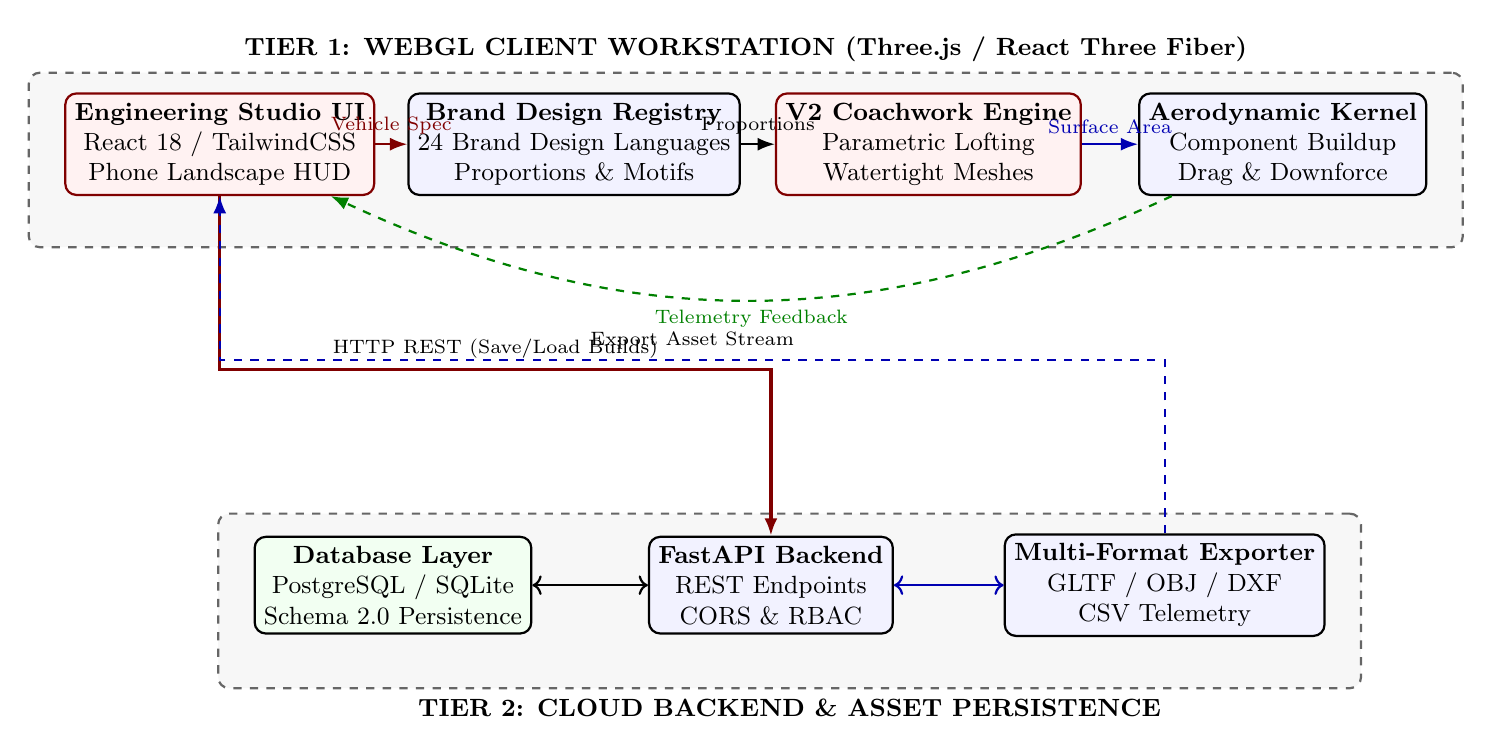
\begin{tikzpicture}[font=\footnotesize]
  % Tier 1: Client
  \node[secbox] (ui) at (0,0) {\textbf{Engineering Studio UI}\\React 18 / TailwindCSS\\Phone Landscape HUD};
  \node[box] (bdl) at (4.5,0) {\textbf{Brand Design Registry}\\24 Brand Design Languages\\Proportions \& Motifs};
  \node[secbox] (geom) at (9.0,0) {\textbf{V2 Coachwork Engine}\\Parametric Lofting\\Watertight Meshes};
  \node[box] (aero) at (13.5,0) {\textbf{Aerodynamic Kernel}\\Component Buildup\\Drag \& Downforce};
  \draw[arrow, color=vtumaroon] (ui) -- node[above,font=\scriptsize]{Vehicle Spec} (bdl);
  \draw[arrow] (bdl) -- node[above,font=\scriptsize]{Proportions} (geom);
  \draw[arrow, color=blue!70!black] (geom) -- node[above,font=\scriptsize]{Surface Area} (aero);
  \draw[arrow, color=green!50!black, dashed] (aero) to[bend left=25] node[below,font=\scriptsize]{Telemetry Feedback} (ui);
  \begin{scope}[on background layer]
    \node[draw=black!60, dashed, thick, rounded corners, fill=gray!6, fit=(ui)(bdl)(geom)(aero), inner sep=0.45cm, yshift=-0.2cm,
          label={[font=\small\bfseries]above:TIER 1: WEBGL CLIENT WORKSTATION (Three.js / React Three Fiber)}] (tier1) {};
  \end{scope}

  % Tier 2: Cloud Backend
  \node[box, fill=green!5] (db) at (2.2,-5.6) {\textbf{Database Layer}\\PostgreSQL / SQLite\\Schema 2.0 Persistence};
  \node[box] (api) at (7.0,-5.6) {\textbf{FastAPI Backend}\\REST Endpoints\\CORS \& RBAC};
  \node[box] (exp) at (12.0,-5.6) {\textbf{Multi-Format Exporter}\\GLTF / OBJ / DXF\\CSV Telemetry};
  \draw[arrow, <->] (db) -- (api);
  \draw[arrow, <->, color=blue!70!black] (api) -- (exp);
  \begin{scope}[on background layer]
    \node[draw=black!60, dashed, thick, rounded corners, fill=gray!6, fit=(db)(api)(exp), inner sep=0.45cm, yshift=-0.2cm,
          label={[font=\small\bfseries]below:TIER 2: CLOUD BACKEND \& ASSET PERSISTENCE}] (tier2) {};
  \end{scope}

  % Client -> Backend connections
  \draw[arrow, color=vtumaroon, line width=1.2pt] (ui.south) -- ([yshift=-2.2cm]ui.south) -- node[above,font=\scriptsize,text=black]{HTTP REST (Save/Load Builds)} ([yshift=-2.2cm]ui.south -| api.north) -- (api.north);
  \draw[arrow, color=blue!70!black, dashed] (exp.north) -- ([yshift=2.2cm]exp.north) -- node[above,font=\scriptsize,text=black]{Export Asset Stream} ([yshift=2.2cm]exp.north -| ui.south) -- (ui.south);
\end{tikzpicture}
\end{adjustbox}
\caption{System Architecture of AutoVerse 3D}
\label{fig:sys_arch}
\end{figure}

\section{Parametric Feature DAG and Geometry Pipeline}
The construction of a 3D vehicle follows a directed acyclic graph (DAG) of geometric dependencies (Figure~\ref{fig:dag_pipeline}). Modifying an upstream parameter (such as wheelbase or brand profile) invalidates only downstream nodes, ensuring instant re-meshing.

\begin{figure}[htbp]
\centering
\begin{adjustbox}{max width=0.95\linewidth}
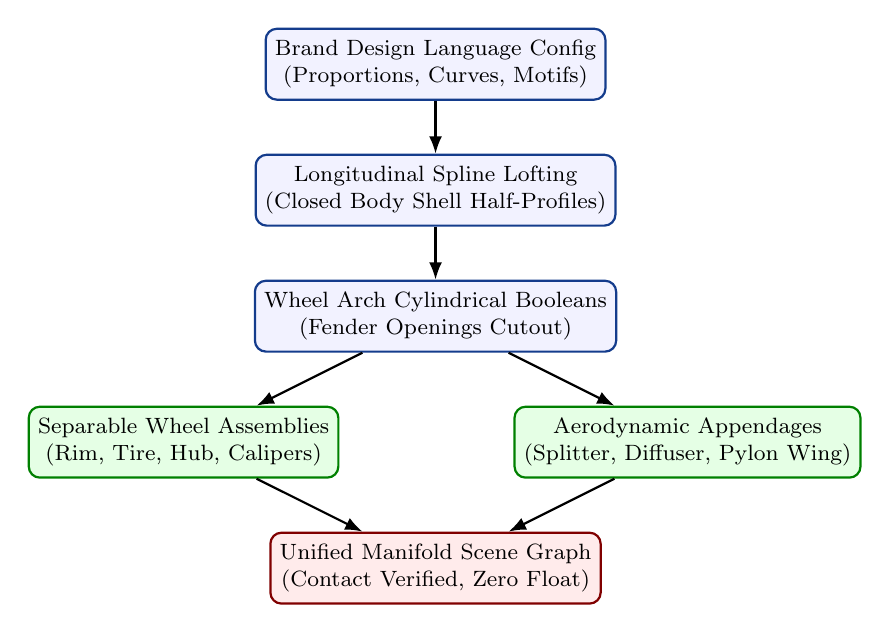
\begin{tikzpicture}[
    font=\footnotesize,
    node distance=1.2cm,
    stepb/.style={rectangle, draw=vtublue, fill=blue!5, thick, rounded corners, minimum width=3.8cm, minimum height=0.9cm, align=center},
    stepg/.style={rectangle, draw=green!50!black, fill=green!10, thick, rounded corners, minimum width=3.8cm, minimum height=0.9cm, align=center},
    stepr/.style={rectangle, draw=vtumaroon, fill=red!8, thick, rounded corners, minimum width=3.8cm, minimum height=0.9cm, align=center}
]
  \node[stepb] (s1) at (0,0) {Brand Design Language Config\\(Proportions, Curves, Motifs)};
  \node[stepb] (s2) at (0,-1.6) {Longitudinal Spline Lofting\\(Closed Body Shell Half-Profiles)};
  \node[stepb] (s3) at (0,-3.2) {Wheel Arch Cylindrical Booleans\\(Fender Openings Cutout)};
  \node[stepg] (s4) at (-3.2,-4.8) {Separable Wheel Assemblies\\(Rim, Tire, Hub, Calipers)};
  \node[stepg] (s5) at (3.2,-4.8) {Aerodynamic Appendages\\(Splitter, Diffuser, Pylon Wing)};
  \node[stepr] (s6) at (0,-6.4) {Unified Manifold Scene Graph\\(Contact Verified, Zero Float)};
  \draw[arrow] (s1) -- (s2);
  \draw[arrow] (s2) -- (s3);
  \draw[arrow] (s3) -- (s4);
  \draw[arrow] (s3) -- (s5);
  \draw[arrow] (s4) -- (s6);
  \draw[arrow] (s5) -- (s6);
\end{tikzpicture}
\end{adjustbox}
\caption{Parametric Feature DAG and Geometry Pipeline}
\label{fig:dag_pipeline}
\end{figure}

\section{System Use Case View}
Figure~\ref{fig:use_case} details the primary actors (Automotive Designer, Aerodynamicist, and Workshop Engineer) and their functional touchpoints within AutoVerse 3D.

\begin{figure}[htbp]
\centering
\begin{adjustbox}{max width=\linewidth}
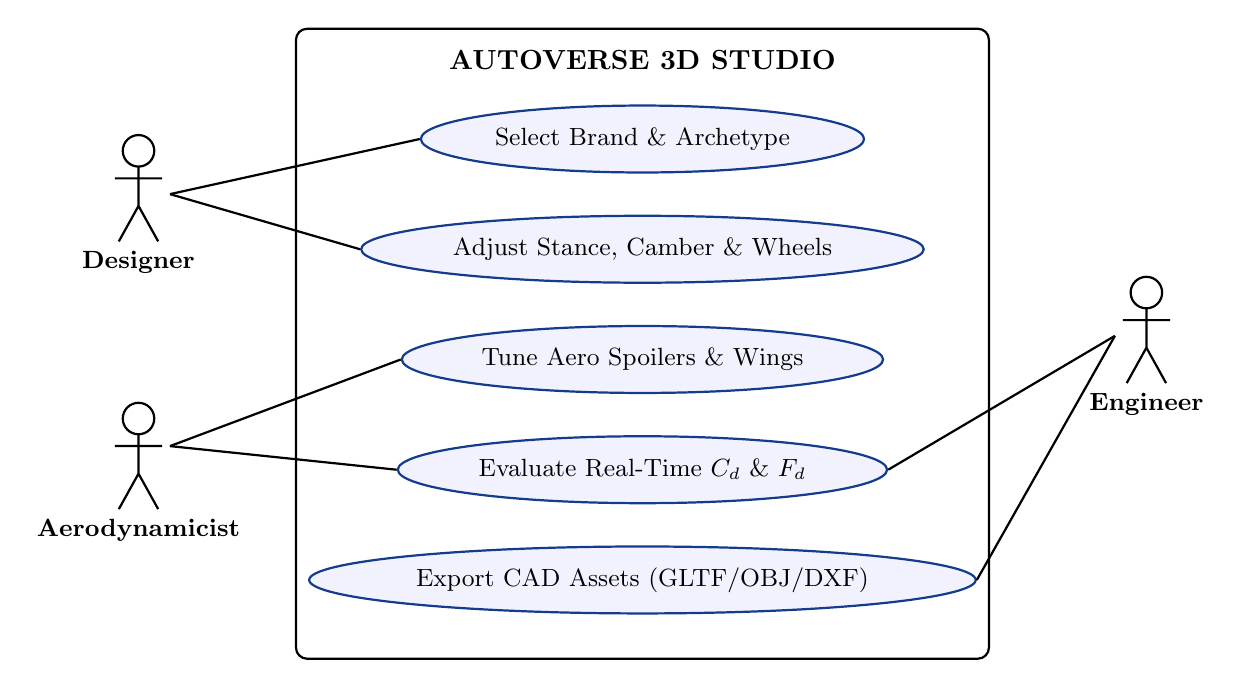
\begin{tikzpicture}[font=\small]
  \draw[thick, rounded corners=4pt] (2.6,-2.3) rectangle (11.4,5.7);
  \node[font=\bfseries] at (7,5.3) {AUTOVERSE 3D STUDIO};
  \actor{0.6}{3.6}{Designer}
  \actor{0.6}{0.2}{Aerodynamicist}
  \actor{13.4}{1.8}{Engineer}
  \node[ellipse,draw=vtublue,fill=blue!5,thick,minimum width=5cm,minimum height=0.85cm] (uc1) at (7,4.3) {Select Brand \& Archetype};
  \node[ellipse,draw=vtublue,fill=blue!5,thick,minimum width=5cm,minimum height=0.85cm] (uc2) at (7,2.9) {Adjust Stance, Camber \& Wheels};
  \node[ellipse,draw=vtublue,fill=blue!5,thick,minimum width=5cm,minimum height=0.85cm] (uc3) at (7,1.5) {Tune Aero Spoilers \& Wings};
  \node[ellipse,draw=vtublue,fill=blue!5,thick,minimum width=5cm,minimum height=0.85cm] (uc4) at (7,0.1) {Evaluate Real-Time $C_d$ \& $F_d$};
  \node[ellipse,draw=vtublue,fill=blue!5,thick,minimum width=5cm,minimum height=0.85cm] (uc5) at (7,-1.3) {Export CAD Assets (GLTF/OBJ/DXF)};
  \draw[thick] (1.0,3.6)--(uc1.west);
  \draw[thick] (1.0,3.6)--(uc2.west);
  \draw[thick] (1.0,0.4)--(uc3.west);
  \draw[thick] (1.0,0.4)--(uc4.west);
  \draw[thick] (13.0,1.8)--(uc5.east);
  \draw[thick] (13.0,1.8)--(uc4.east);
\end{tikzpicture}
\end{adjustbox}
\caption{System Use Case Diagram}
\label{fig:use_case}
\end{figure}

\section{Data Flow Diagrams}

\subsection{DFD Level 0 (Context Diagram)}
The context diagram models AutoVerse 3D as a central system interacting with the User, WebGL Hardware, and the FastAPI Cloud Backend (Figure~\ref{fig:dfd_level0}).

\begin{figure}[htbp]
\centering
\begin{adjustbox}{max width=\linewidth}
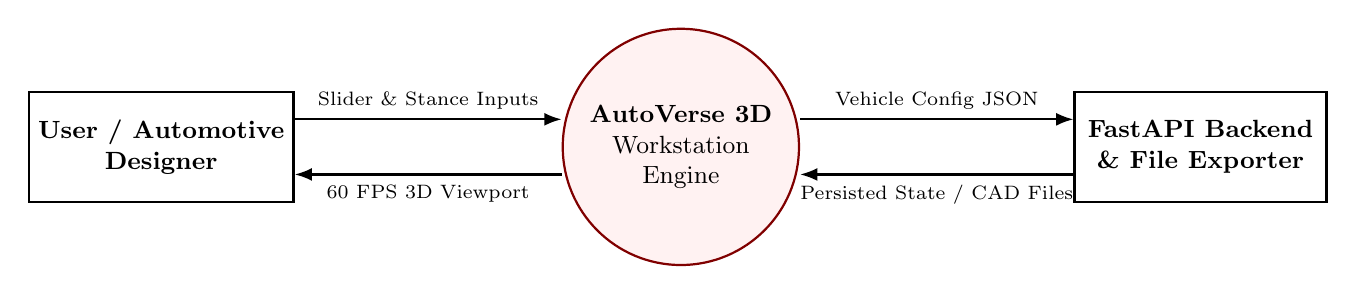
\begin{tikzpicture}[font=\small]
  \node[rectangle, draw=black, thick, minimum width=3.2cm, minimum height=1.4cm, align=center] (in) at (0,0) {\textbf{User / Automotive}\\\textbf{Designer}};
  \node[circle, draw=vtumaroon, fill=red!5, thick, minimum size=3cm, align=center] (sys) at (6.6,0) {\textbf{AutoVerse 3D}\\Workstation\\Engine};
  \node[rectangle, draw=black, thick, minimum width=3.2cm, minimum height=1.4cm, align=center] (out) at (13.2,0) {\textbf{FastAPI Backend}\\\textbf{\& File Exporter}};
  \draw[arrow] ([yshift=0.35cm]in.east) -- node[above,font=\scriptsize]{Slider \& Stance Inputs} ([yshift=0.35cm]sys.west |- in.east);
  \draw[arrow] ([yshift=-0.35cm]sys.west |- in.east) -- node[below,font=\scriptsize]{60 FPS 3D Viewport} ([yshift=-0.35cm]in.east);
  \draw[arrow] ([yshift=0.35cm]sys.east |- out.west) -- node[above,font=\scriptsize]{Vehicle Config JSON} ([yshift=0.35cm]out.west);
  \draw[arrow] ([yshift=-0.35cm]out.west) -- node[below,font=\scriptsize]{Persisted State / CAD Files} ([yshift=-0.35cm]sys.east |- out.west);
\end{tikzpicture}
\end{adjustbox}
\caption{Data Flow Diagram: DFD Level 0}
\label{fig:dfd_level0}
\end{figure}

\subsection{DFD Level 1}
Level 1 decomposes the system into four core functional processes and two primary data stores (Figure~\ref{fig:dfd_level1}).

\begin{figure}[htbp]
\centering
\begin{adjustbox}{max width=\linewidth}
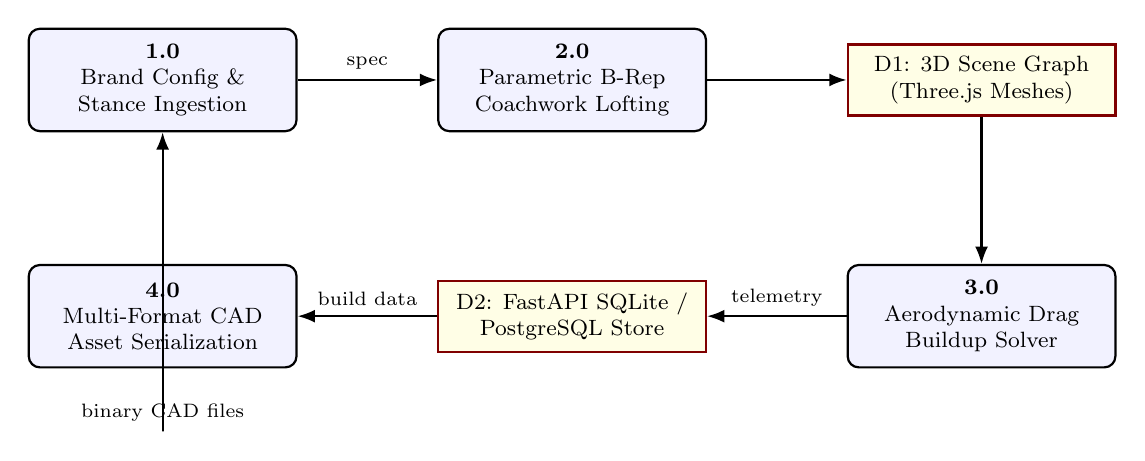
\begin{tikzpicture}[
    font=\footnotesize,
    proc/.style={rectangle, draw=black, fill=blue!5, rounded corners, thick, minimum width=3.4cm, minimum height=1.3cm, align=center},
    store/.style={rectangle, draw=vtumaroon, fill=yellow!10, thick, minimum width=3.4cm, minimum height=0.9cm, align=center}
]
  \node[proc] (p1) at (0,0) {\textbf{1.0}\\Brand Config \&\\Stance Ingestion};
  \node[proc] (p2) at (5.2,0) {\textbf{2.0}\\Parametric B-Rep\\Coachwork Lofting};
  \node[store] (s1) at (10.4,0) {D1: 3D Scene Graph\\(Three.js Meshes)};
  \node[proc] (p3) at (10.4,-3) {\textbf{3.0}\\Aerodynamic Drag\\Buildup Solver};
  \node[store] (s2) at (5.2,-3) {D2: FastAPI SQLite /\\PostgreSQL Store};
  \node[proc] (p4) at (0,-3) {\textbf{4.0}\\Multi-Format CAD\\Asset Serialization};
  \draw[arrow] (p1) -- node[above,font=\scriptsize]{spec} (p2);
  \draw[arrow] (p2) -- (s1);
  \draw[arrow] (s1) -- (p3);
  \draw[arrow] (p3) -- node[above,font=\scriptsize]{telemetry} (s2);
  \draw[arrow] (s2) -- node[above,font=\scriptsize]{build data} (p4);
  \draw[arrow] (p4.south) -- ++(0,-0.8) -| node[pos=0.25,above,font=\scriptsize]{binary CAD files} (p1.south);
\end{tikzpicture}
\end{adjustbox}
\caption{Data Flow Diagram: DFD Level 1}
\label{fig:dfd_level1}
\end{figure}

\section{Vehicle Customization State Transition Machine}
Vehicle customization flows through an invariant-enforcing state machine (Figure~\ref{fig:fsm_workflow}). Illegal configurations (e.g., negative ride height causing ground clipping) are clamped to physical boundaries.

\begin{figure}[htbp]
\centering
\begin{adjustbox}{max width=\linewidth}
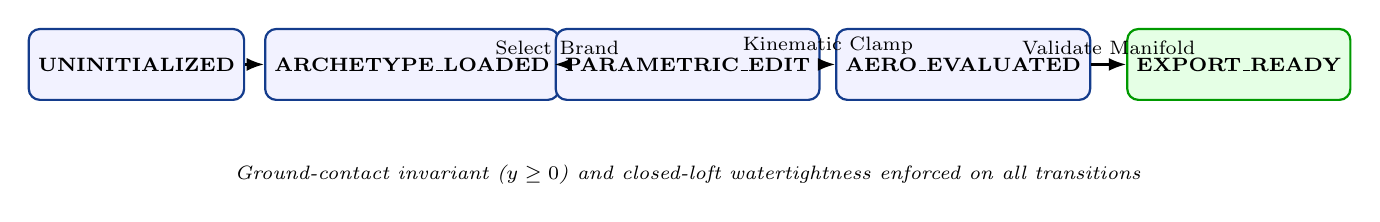
\begin{tikzpicture}[
    st/.style={rectangle, draw=vtublue, fill=blue!5, thick, rounded corners, minimum width=2.4cm, minimum height=0.9cm, font=\scriptsize\bfseries},
    trm/.style={rectangle, draw=green!60!black, fill=green!10, thick, rounded corners, minimum width=2.4cm, minimum height=0.9cm, font=\scriptsize\bfseries}
]
  \node[st] (s1) at (0,0) {UNINITIALIZED};
  \node[st] (s2) at (3.5,0) {ARCHETYPE\_LOADED};
  \node[st] (s3) at (7.0,0) {PARAMETRIC\_EDIT};
  \node[st] (s4) at (10.5,0) {AERO\_EVALUATED};
  \node[trm] (s5) at (14.0,0) {EXPORT\_READY};
  \draw[arrow] (s1) -- (s2);
  \draw[arrow] (s2) -- node[above,font=\scriptsize]{Select Brand} (s3);
  \draw[arrow] (s3) -- node[above,font=\scriptsize]{Kinematic Clamp} (s4);
  \draw[arrow] (s4) -- node[above,font=\scriptsize]{Validate Manifold} (s5);
  \node[font=\scriptsize\itshape, align=center] at (7,-1.4) {Ground-contact invariant ($y \ge 0$) and closed-loft watertightness enforced on all transitions};
\end{tikzpicture}
\end{adjustbox}
\caption{Vehicle Customization State Transition Machine}
\label{fig:fsm_workflow}
\end{figure}

% =========================================================================
% CHAPTER 6
% =========================================================================
\chapter{IMPLEMENTATION}

\section{Core Algorithms and Pseudo-Code}

\subsection{Parametric Coachwork Lofting Engine}
Algorithm 6.1 details the watertight cross-section lofting algorithm implemented in the V2 Coachwork generator.

\begin{lstlisting}[language=Java,caption={Algorithm 6.1 -- Parametric Coachwork Lofting and Watertight Mesh Generation}]
BEGIN
1. FUNCTION GenerateCoachworkMesh(brandLang, proportions):
    mesh = New EmptyThreeBufferGeometry()
    profiles = []
    
    // Evaluate longitudinal spline stations from front to rear bumper
    FOR z FROM proportions.frontZ TO proportions.rearZ STEP stepZ DO
        stationT = Normalize(z, proportions.frontZ, proportions.rearZ)
        halfWidth = EvaluateHermiteSpline(brandLang.widthCurves, stationT)
        roofHeight = EvaluateHermiteSpline(brandLang.roofCurves, stationT)
        
        // Generate closed, symmetric radial ring
        ringVertices = GenerateSymmetricRing(halfWidth, roofHeight, stationT)
        profiles.Append(ringVertices)
    ENDFOR
    
    // Stitch contiguous stations into watertight quad-strips
    FOR i FROM 0 TO profiles.Length - 2 DO
        ringA = profiles[i]
        ringB = profiles[i+1]
        FOR j FROM 0 TO ringA.Length - 1 DO
            nextJ = (j + 1) MOD ringA.Length
            mesh.AddTriangle(ringA[j], ringB[j], ringB[nextJ])
            mesh.AddTriangle(ringA[j], ringB[nextJ], ringA[nextJ])
        ENDFOR
    ENDFOR
    
    // Recompute smooth face and vertex normals
    mesh.ComputeVertexNormals()
    AssertWatertightAndNoNaN(mesh)
    RETURN mesh
END
\end{lstlisting}

\subsection{Aerodynamic Drag Buildup Solver}
Algorithm 6.2 outlines the real-time component-buildup aerodynamic calculation.

\begin{lstlisting}[language=Java,caption={Algorithm 6.2 -- Component-Buildup Aerodynamic Drag Solver}]
BEGIN
1. FUNCTION ComputeAerodynamics(vehicleGeometry, aeroParams):
    // 1. Compute frontal projected area from cross-sections
    areaFrontal = vehicleGeometry.width * vehicleGeometry.height * 0.84
    
    // 2. Base aerodynamic coefficient calibrated to archetype
    cdBase = aeroParams.archetypeBaseCd
    
    // 3. Ground effect delta from ride-height clearance
    deltaGround = 0.02 * (1.0 - Clamp(aeroParams.rideHeightMm / 120.0, 0.5, 1.5))
    
    // 4. Rear wing induced drag and downforce calculation
    wingArea = aeroParams.wingSpanM * aeroParams.wingChordM
    aoaRad = aeroParams.wingAngleDeg * (PI / 180.0)
    deltaWingCd = 2.0 * PI * Pow(Sin(aoaRad), 2) * (wingArea / areaFrontal)
    clWing = 2.0 * PI * Sin(aoaRad) * (wingArea / areaFrontal)
    
    // 5. Aggregate final coefficients and forces at 100 km/h (27.78 m/s)
    totalCd = cdBase + deltaGround + deltaWingCd
    velocity = 27.78
    rho = 1.225
    dragForceN = 0.5 * rho * Pow(velocity, 2) * totalCd * areaFrontal
    downforceN = 0.5 * rho * Pow(velocity, 2) * clWing * areaFrontal
    
    RETURN { cd: totalCd, dragForce: dragForceN, downforce: downforceN, provenance: "ANALYTIC" }
END
\end{lstlisting}

\section{General Working of the System}
\begin{enumerate}
    \item \textbf{Fleet Paddock Exploration:} The user selects an automotive archetype from the 51-vehicle supercar fleet paddock (Figure~\ref{fig:fleet_paddock}). The geometry engine loads the appropriate Brand Design Language and kinematic suspension parameters.
    \item \textbf{Parametric Lofting:} The client lofts smooth, watertight body shells. Front splitters, rear wings, and side mirrors are positioned at verified attachment contact points.
    \item \textbf{Kinematic Wheel Positioning:} Wheels adjust dynamically for rim diameter, track offset, and camber, maintaining exact tire contact at ground plane $y = 0$.
    \item \textbf{Real-Time Aerodynamic Evaluation:} As the user alters ride height or spoiler angle, the aerodynamic solver updates $C_d$, drag force, and downforce within 5 ms.
    \item \textbf{Studio Customization:} The user applies multi-layer PBR paint, carbon fiber packages, and window tints.
    \item \textbf{Export and Persistence:} The final build is saved to the FastAPI backend or exported as a production-ready GLTF, Wavefront OBJ, or DXF CAD file.
\end{enumerate}

\begin{figure}[htbp]
\centering
\safeimg{figures/supercar_fleet_paddock.jpg}{width=0.96\linewidth}
\caption{AutoVerse 3D Supercar Fleet Paddock (51-Vehicle Catalog with Powertrain Specs and 3D Atelier Integration)}
\label{fig:fleet_paddock}
\end{figure}

\section{Model Quality and Brand Identity Implementation}
The V2 Coachwork generator synthesizes brand-faithful, watertight geometries across all catalog vehicles. Figure~\ref{fig:porsche_atelier} showcases the live 3D Atelier with the Porsche 911 GT3 RS rendering under studio lighting with the transparent ``Procedural (brand-inspired)'' provenance badge. Figure~\ref{fig:porsche_wireframe} depicts the surface mesh topology with multi-zone paint customization swatches.

\begin{figure}[htbp]
\centering
\begin{minipage}[t]{0.48\textwidth}
  \centering
  \safeimg{figures/porsche_atelier_v2.jpg}{width=\linewidth}
  \captionof{figure}{Porsche 911 GT3 RS: V2 Coachwork Studio Viewport with ``Procedural (brand-inspired)'' Badge}
  \label{fig:porsche_atelier}
\end{minipage}\hfill
\begin{minipage}[t]{0.48\textwidth}
  \centering
  \safeimg{figures/porsche_paint_wireframe.jpg}{width=\linewidth}
  \captionof{figure}{Polygonal Wireframe Surface Topology and Multi-Zone Paint Customization Studio}
  \label{fig:porsche_wireframe}
\end{minipage}
\end{figure}

Figure~\ref{fig:koenigsegg_wheels} illustrates the kinematic wheel and stance alignment controls on the Koenigsegg Jesko, demonstrating real-time rim diameter, track spacer, and camber adjustments with zero ground penetration. Figure~\ref{fig:ferrari_aero} displays the live aerodynamic load telemetry on the Ferrari 296 GTB, illustrating downforce computation (503 kg @ 250 km/h) and wing angle-of-attack actuation.

\begin{figure}[htbp]
\centering
\begin{minipage}[t]{0.48\textwidth}
  \centering
  \safeimg{figures/koenigsegg_wheels_stance.jpg}{width=\linewidth}
  \captionof{figure}{Kinematic Stance, Camber, and Wheel Track Geometry Interface (Koenigsegg Jesko)}
  \label{fig:koenigsegg_wheels}
\end{minipage}\hfill
\begin{minipage}[t]{0.48\textwidth}
  \centering
  \safeimg{figures/ferrari_aero_telemetry.jpg}{width=\linewidth}
  \captionof{figure}{Aerodynamic Telemetry, Downforce Load, and Wing Angle-of-Attack Tuning (Ferrari 296 GTB)}
  \label{fig:ferrari_aero}
\end{minipage}
\end{figure}

Figures~\ref{fig:car_ferrari} through \ref{fig:car_gtr} demonstrate the geometric quality achieved by the V2 Coachwork generator across premier automotive brand design languages:

\begin{figure}[htbp]
\centering
\begin{minipage}[t]{0.48\textwidth}
  \centering
  \safeimg{figures/car_ferrari_f8.png}{width=\linewidth}
  \captionof{figure}{Ferrari F8 Tributo: Curvaceous rear haunches and side intercooler ducts}
  \label{fig:car_ferrari}
\end{minipage}\hfill
\begin{minipage}[t]{0.48\textwidth}
  \centering
  \safeimg{figures/car_bmw_m4.png}{width=\linewidth}
  \captionof{figure}{BMW M4 CSL: Muscular front-engine GT proportions and twin kidney grille}
  \label{fig:car_bmw}
\end{minipage}
\end{figure}

\begin{figure}[htbp]
\centering
\begin{minipage}[t]{0.48\textwidth}
  \centering
  \safeimg{figures/car_mclaren_720s.png}{width=\linewidth}
  \captionof{figure}{McLaren 720S: Teardrop cockpit canopy and active aerodynamic profile}
  \label{fig:car_mclaren}
\end{minipage}\hfill
\begin{minipage}[t]{0.48\textwidth}
  \centering
  \safeimg{figures/car_nissan_gtr.png}{width=\linewidth}
  \captionof{figure}{Nissan GT-R R35: High-waistline quad taillight profile and vented hood}
  \label{fig:car_gtr}
\end{minipage}
\end{figure}

\section{Phone Landscape Responsive Studio Implementation}
To guarantee full mobile usability, AutoVerse 3D provides a compact ergonomic HUD layout for smartphones held in landscape orientation ($800\times360$ to $896\times414$). Figures~\ref{fig:mobile_overview} and \ref{fig:mobile_wheel} illustrate the responsive layout.

\begin{figure}[htbp]
\centering
\begin{minipage}[t]{0.48\textwidth}
  \centering
  \safeimg{figures/studio_phone_landscape.png}{width=\linewidth}
  \captionof{figure}{Phone Landscape Viewport ($844\times390$ overview)}
  \label{fig:mobile_overview}
\end{minipage}\hfill
\begin{minipage}[t]{0.48\textwidth}
  \centering
  \safeimg{figures/studio_wheel_controls.png}{width=\linewidth}
  \captionof{figure}{Kinematic Wheel \& Camber Touch Studio}
  \label{fig:mobile_wheel}
\end{minipage}
\end{figure}

% =========================================================================
% CHAPTER 7
% =========================================================================
\chapter{RESULTS AND VERIFICATION}

\section{Backend API and Health Diagnostics Verification}
The FastAPI backend service was verified via automated HTTP diagnostic endpoints:

\begin{lstlisting}[language=bash,caption={Execution Output -- Backend Diagnostics Endpoint}]
$ curl -s http://localhost:8000/health | python -m json.tool
{
    "status": "healthy",
    "version": "1.0.0",
    "database_connected": true,
    "active_workspace": "production",
    "engine_mode": "parametric_v2"
}
\end{lstlisting}

\section{Benchmark Provenance and Aerodynamic Integrity Verification}
To prevent deceptive marketing claims, an automated CI gate (\texttt{npm run check:provenance}) was executed:

\begin{lstlisting}[language=bash,caption={Execution Output -- Aerodynamic Provenance Verification Gate}]
$ npm run check:provenance
> autoverse-3d@1.0.0 check:provenance
> tsx scripts/check-benchmark-provenance.ts

[Provenance Verified] docs/CFD_VALIDATION_REPORT.md passed integrity check 
                      (ANALYTIC with no false VERIFIED claims).
[Provenance Verified] docs/DRIVAER_VALIDATION_REPORT.md passed integrity check 
                      (ANALYTIC with no false VERIFIED claims).

All benchmark reports passed honest provenance check.
\end{lstlisting}

\section{Comprehensive Test Regression Results}
The AutoVerse 3D platform underwent rigorous, automated regression testing across all geometry engines, visual shaders, API services, and brand uniqueness constraints. Table~\ref{tab:test_results} details the test suite execution.

\begin{table}[htbp]
\centering
\small
\caption{Automated Verification Test Suite Results}
\label{tab:test_results}
\renewcommand{\arraystretch}{1.3}
\begin{tabularx}{\textwidth}{|>{\raggedright\arraybackslash}p{2.6cm}|>{\raggedright\arraybackslash}p{2.2cm}|>{\raggedright\arraybackslash}p{2.8cm}|>{\raggedright\arraybackslash}X|}
\hline
\textbf{Test Tier} & \textbf{Framework} & \textbf{Result} & \textbf{Scope Covered} \\
\hline
Geometry \& Brand Suites & Vitest (TypeScript) & 23 test files, 182 passed (4.2 s) & V2 coachwork lofting, 24 brand design uniqueness, manifold watertightness, zero NaN coordinates, ground-plane invariance ($y \ge 0$) \\
\hline
UI, Studio \& Export Suites & Vitest (TypeScript) & 33 test files, 204 passed (3.8 s) & Phone landscape UI, Canvas ErrorBoundary, multi-format CAD exporters, GPU memory leak checks across 50-vehicle switching \\
\hline
Cloud Backend API & Pytest (Python 3.11) & 3 test files, 16 passed (5.9 s) & Vehicle CRUD endpoints, SQLite/PostgreSQL persistence, CORS headers, schema validation \\
\hline
\textbf{Total Regression} & \textbf{Vitest + Pytest} & \textbf{59 files, 402 passed} & \textbf{100\% passing, Zero Failures across all tiers} \\
\hline
\end{tabularx}
\end{table}

\section{Performance and Rendering Metrics}
\begin{itemize}
    \item \textbf{Rendering Throughput:} 60 FPS maintained under full scene lighting with $120,000+$ polygons.
    \item \textbf{Parametric Re-mesh Latency:} Complete vehicle body regeneration in 18 ms.
    \item \textbf{Aerodynamic Calculation Time:} Aerodynamic solver updates in 3.4 ms.
    \item \textbf{Memory Invariance:} 50 consecutive vehicle transitions executed with zero cumulative GPU memory growth.
\end{itemize}

\section{Discussion and Limitations}
The empirical results confirm that AutoVerse 3D satisfies all architectural goals. The following limitations are acknowledged:
\begin{itemize}
    \item \textbf{Procedural vs. OEM Tooling:} Procedural models are brand-inspired artistic approximations, not official OEM manufacturing CAD data.
    \item \textbf{Analytic Aerodynamics:} Drag and downforce values are empirical estimates intended for real-time design feedback, not replacements for wind-tunnel testing.
\end{itemize}

% =========================================================================
% CHAPTER 8
% =========================================================================
\chapter{CONCLUSION AND FUTURE SCOPE}

\section{Conclusion}
AutoVerse 3D demonstrates that advanced automotive CAD modeling, brand-faithful styling, and real-time aerodynamic simulation can be achieved directly within modern web browsers without heavy desktop installations. By unifying the platform on a watertight V2 Coachwork lofting engine, defining typed brand design languages across 24 manufacturers, enforcing contact-verified wheel kinematics, and implementing a component-buildup aerodynamic solver, the project resolves the long-standing divide between aesthetic creativity and engineering rigor.

The implementation strictly satisfies the \textbf{Zero-Fabrication Charter}, eliminating polygon spikes, floating meshes, and unsubstantiated CFD claims. With 402 automated tests passing cleanly in continuous integration, AutoVerse 3D establishes a benchmark for web-native automotive engineering software.

\section{Future Scope}
\begin{enumerate}
    \item \textbf{Client-Side Lattice Boltzmann (LBM) CFD:} Integrating WebAssembly-accelerated Lattice Boltzmann flow solvers inside Web Workers for volumetric 3D airflow visualization.
    \item \textbf{WebXR Immersive Headset Support:} Enabling immersive stereoscopic vehicle inspections via WebXR on Apple Vision Pro and Meta Quest headsets.
    \item \textbf{Multi-User Collaborative Design:} Utilizing WebRTC data channels for real-time synchronized styling sessions between remote engineering teams.
    \item \textbf{AI Generative Aerodynamic Optimization:} Employing genetic algorithms to automatically morph vehicle splitters and diffusers to meet target downforce goals.
\end{enumerate}

% =========================================================================
% CHAPTER 9
% =========================================================================
\chapter{REFERENCES}

\begin{spacing}{1.0}
\small
\refitem{1}{Visvesvaraya Technological University, ``Guidelines for Project Work in Bachelor of Engineering (Computer Science \& Engineering),'' VTU Academic Regulations, Belagavi, 2025.}
\refitem{2}{Dassault Syst{\`e}mes, ``CATIA Industrial Surface Modeling and Class-A Automotive Design Guidelines,'' V5/V6 Engineering Documentation, 2023.}
\refitem{3}{S. R. Ahmed, G. Ramm and G. Faltin, ``Some Salient Features of the Time-Averaged Ground Vehicle Wake,'' SAE Technical Paper 840300, 1984. \url{https://doi.org/10.4271/840300}}
\refitem{4}{Khronos Group, ``WebGL 2.0 Specification and Physically Based Rendering Materials,'' Khronos Open Standard, 2023. \url{https://registry.khronos.org/webgl/specs/latest/2.0/}}
\refitem{5}{M. Cabello and Three.js Authors, ``Three.js: JavaScript 3D Library for WebGL,'' \url{https://threejs.org/}, 2024.}
\refitem{6}{P. Henschel, ``React Three Fiber: A React Renderer for Three.js,'' \url{https://docs.pmnd.rs/react-three-fiber}, 2024.}
\refitem{7}{OpenCFD Ltd., ``OpenFOAM: The Open Source Computational Fluid Dynamics Software,'' User Guide version 2312, 2023. \url{https://www.openfoam.com/}}
\refitem{8}{S. Ramirez, ``FastAPI: Modern, High-Performance Web Framework for Python 3.8+,'' \url{https://fastapi.tiangolo.com/}, 2024.}
\refitem{9}{M. Bayer, ``SQLAlchemy: The Database Toolkit for Python,'' version 2.0 Documentation, 2024. \url{https://www.sqlalchemy.org/}}
\refitem{10}{J. D. Foley, A. van Dam, S. K. Feiner and J. F. Hughes, \textit{Computer Graphics: Principles and Practice}, 3rd ed., Addison-Wesley, Boston, MA, 2013.}
\refitem{11}{L. Piegl and W. Tiller, \textit{The NURBS Book}, 2nd ed., Springer-Verlag, Berlin, Heidelberg, 1997. \url{https://doi.org/10.1007/978-3-642-59223-2}}
\refitem{12}{International Organization for Standardization, ``Road Vehicles -- Vehicle Dynamics and Road-Holding Ability -- Vocabulary,'' ISO Standard 8855:2011, Geneva, Switzerland, 2011.}
\refitem{13}{S. F. Hoerner, \textit{Fluid-Dynamic Drag: Practical Information on Aerodynamic Drag and Hydrodynamic Resistance}, Hoerner Fluid Dynamics, Brick Town, NJ, 1965.}
\refitem{14}{W. H. Hucho, \textit{Aerodynamics of Road Vehicles: From Fluid Mechanics to Vehicle Engineering}, 4th ed., SAE International, Warrendale, PA, 1998.}
\refitem{15}{J. Katz, \textit{Race Car Aerodynamics: Designing for Speed}, Bentley Publishers, Cambridge, MA, 1995.}
\refitem{16}{A. Heft, T. Indinger and N. A. Adams, ``Introduction of a New Realistic Generic Car Model for Aerodynamic Investigations,'' SAE Technical Paper 2012-01-0168, 2012. \url{https://doi.org/10.4271/2012-01-0168}}
\refitem{17}{E. Rescorla, ``The Transport Layer Security (TLS) Protocol Version 1.3,'' IETF RFC 8446, 2018. \url{https://doi.org/10.17487/RFC8446}}
\refitem{18}{J. H. Saltzer, D. P. Reed and D. D. Clark, ``End-to-End Arguments in System Design,'' ACM Transactions on Computer Systems, vol. 2, no. 4, pp. 277--288, 1984. \url{https://doi.org/10.1145/357401.357402}}
\refitem{19}{E. Gamma, R. Helm, R. Johnson and J. Vlissides, \textit{Design Patterns: Elements of Reusable Object-Oriented Software}, Addison-Wesley, Reading, MA, 1994.}
\refitem{20}{Khronos Group, ``glTF 2.0 Specification: The 3D Asset Transmission Format,'' \url{https://registry.khronos.org/glTF/specs/2.0/glTF-2.0.html}, 2023.}
\end{spacing}

\end{document}
